\chapter{COFFEE: a Compiler for Fast Expression Evaluation}
\label{ch:coffee}

\section{Overview}
Sharing elimination and pre-evaluation, which we presented in Chapter~\ref{ch:optimality}, as well as the low level optimizations discussed in Chapter~\ref{ch:lowlevelopt}, have been implemented in COFFEE\footnote{COFFEE is the acronym for COmpiler For Fast Expression Evaluation.}, a mature, platform-agnostic compiler. COFFEE has fully been integrated with Firedrake, the framework for finite element methods introduced in Section~\ref{sec:bkg:firedrake}. The code, which comprises more than 5000 lines, is available at~\citep{coffee-code}.

Firedrake users employ the Unified Form Language to express problems in a notation resembling mathematical equations. At run-time, the high-level specification is translated by a form compiler, the Two-Stage Form Compiler (TSFC)~\cite{TSFC-Compiler}, into one or more abstract syntax trees (ASTs) representing assembly kernels. ASTs are then passed to COFFEE for optimization. The output of COFFEE, C code, is eventually provided to PyOP2~\citep{pyop2isc}, where just-in-time compilation and execution over the discretized domain take place. The flow and the compiler structure are outlined in Figure~\ref{fig:coffee-pipeline}. 

\begin{figure}
\begin{center}
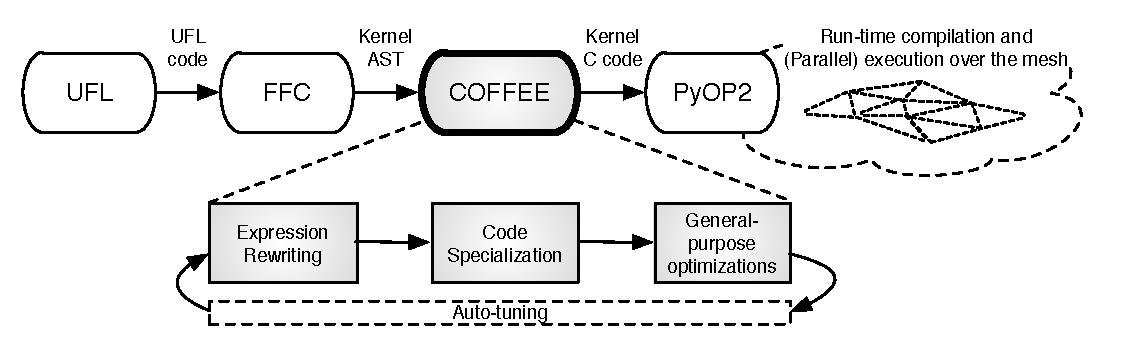
\includegraphics[scale=0.70]{coffee/pictures/coffee-pipeline.pdf}
\caption{High-level view of Firedrake. COFFEE is at the core, receiving ASTs from a modified version of the FEniCS Form Compiler and producing optimized C code kernels.}
\label{fig:coffee-pipeline}
\end{center}
\end{figure}

\section{The Optimization Pipeline}
Similarly to general-purpose compilers, COFFEE provides different optimization levels, namely \texttt{O0}, \texttt{O1}, \texttt{O2} and \texttt{O3}. Apart from \texttt{O0}, which does not transform the code received from the form compiler (useful for debugging purposes), all optimization levels apply ordered sequences of optimizations. In essence, the higher the optimization level, the more aggressive (and potentially slower) is the transformation process. There also are aspects of the optimization process that are common to \texttt{O1}, \texttt{O2} and \texttt{O3}; in the following, when describing them, we will use the generic notation \texttt{Ox} (\texttt{x} $\in \lbrace 1, 2, 3\rbrace$).

The optimization level \texttt{Ox} can logically be split into three phases:
\begin{description}
\item[Expression rewriting] Any transformation changing the structure of the expressions (and, potentially, of the loop nests) in the assembly kernel. For example, a high level optimization (sharing elimination, pre-evaluation) or, more in general, any rewrite operator (described later in Section~\ref{sec:coffee:rewrite-ops}) such as generalized code motion or factorization. 
\item[Handling of block-sparse tables] Explained in Section~\ref{ch:optimality:block-sparse}, this phase consists of restructuring the iteration spaces searching for a trade-off between avoidance of useless operations involving blocks of zeros in basis function tables and effectiveness of low level optimization.
\item[Code Specialization] Low level optimization, tailored to the underlying architecture. The primary focus of this thesis has been conventional CPUs, although a generalization to other platforms is possible. In this phase, a specific combination of the transformations presented in Chapter~\ref{ch:coffee} is applied.
\end{description}
These three phases are totally ordered. Expression rewriting introduces temporaries and creates loops. These new loops, and the statements therein, may further be transformed in the subsequent phase, for instance by adjusting bounds and by introducing memory offsets. In the last phase, both temporaries and loops may be modified by padding and data alignment, vector-register tiling and vector promotion.

When provided to COFFEE, an AST is visited and several kinds of information are collected. In particular, COFFEE searches for special ``expression nodes''. Expression nodes are the candidates for expression rewriting. If we had to represent an expression node in plain C, we could think of it as a (usually compute-intensive) statement preceded by a special \texttt{$\#$pragma coffee expression}; the \texttt{pragma} would then trigger COFFEE's \texttt{Ox}, similarly to the way loops are parallelized in OpenMP. If at least one expression node is found, we proceed to the next step, otherwise the AST is unparsed and C code returned.

In addition to selecting \texttt{Ox}, users can create their own custom optimization pipelines by composing the individual transformations available in COFFEE. For this reason, and since some of the transformations are not composable (because either unsupported or illegal), the second step of the compiler consists of checking the validity of the optimization process. 

At this point, the AST is transformed according to the optimization pipeline. 
\begin{description}
\item[\texttt{O1}] At lowest optimization level, expression rewriting reduces to generalized code motion, while only padding and data alignment are applied among the lower level optimizations.
\item[\texttt{O2}] With respect to \texttt{O1}, there is only one yet fundamental change: expression rewriting now performs sharing elimination (i.e., Algorithm~\ref{algo:sharing-elimination}).
\item[\texttt{O3}] Algorithm~\ref{algo:gamma}, which coordinates sharing elimination and pre-evaluation, is applied. This is followed by handling of block-sparse tables, and finally by padding and data alignment. 
\end{description}
The dichotomy between \texttt{O2} and \texttt{O3} is elaborated in the next section.

Once all optimizations have been applied, the AST is visited one last time and a C representation (a string) is returned.

\section{Plugging COFFEE into Firedrake}
\label{sec:coffee-implementation}

\subsection{Abstract Syntax Trees}
...

\subsection{Integration with the FEniCS Form Compiler}
COFFEE expects as input either a string of C code or an AST. In the former case, a parser could be used to obtain an AST representation, which is required by the algorithms implementing the various code transformations. Therefore, FFC's output, which is a C-code implementation of a local assembly kernel, could be used straightforwardly as input to COFFEE. However, we note that this would also be conceptually pointless: FFC would generate C code from its intermediate representation that eventually COFFEE would have to re-parse to obtain an AST. A much cleaner solution, adopted and explained next, consists of modifying FFC to directly generate an AST. 

The construction of the FFC's intermediate representation from UFL code is refined as follows:
\begin{itemize}
\item The mathematical expression that evaluates the element matrix is represented by a tree data structure. A limitation of the original FFC was that nodes in such expression tree, which correspond to symbols or arithmetic operations, are not bound to the enclosing loops. For instance, consider the symbol \texttt{A[i][j]}: the FFC's expression tree has a node for this symbol, but visiting it there is no clean way of separating the variable name \texttt{A} from the loop indices \texttt{i} and \texttt{j}. Therefore, we have enriched symbol nodes with additional fields to capture these information. 
\item Basis functions in the FFC's intermediate representation are characterized by a new field telling whether they originated from a vector-valued or a scalar-valued element. In the former case, the array rappresenting the tabulation of a basis function at the various quadrature points is block-sparse. This information is recorded and, as explained next, attached to the kernel's AST to enable COFFEE applying symbolic execution to avoid iteration over zero-valued blocks, as elaborated in Section~\ref{sec:coffee-avoidzeros}.
\end{itemize}
In the modified FFC, the intermediate representation is intercepted prior to the code generation stage and forwarded to a new module that builds ASTs. To this purpose, COFFEE exposes its hierarchy of AST nodes, whose design strictly adhere to standard object-oriented programming rules (e.g. by making extensive use of overloading). An example of such an AST representation for a simple C statement is provided in Figure~\ref{fig:coffee-ast-vs-c}.

\begin{figure}
\begin{center}
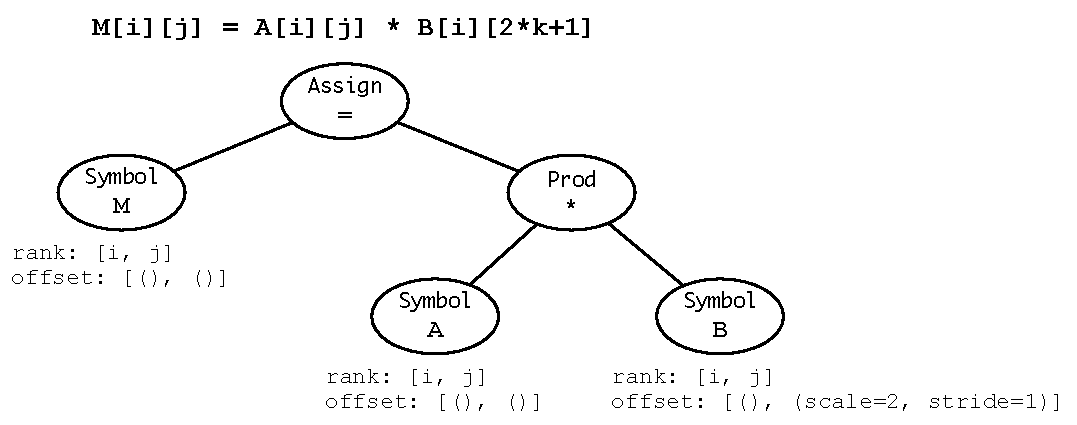
\includegraphics[scale=0.50]{coffee/pictures/coffee-ast.pdf}
\caption{AST representation of a C assignment in COFFEE.}
\label{fig:coffee-ast-vs-c}
\end{center}
\end{figure}

The enriched intermediate representation allows to create proper AST's Symbol nodes. A Symbol, as shown in the figure, has a name (the variable name), an array of indices, and an array of offsets. These information are fundamental for the implementation of expression rewriting and code specialization. Further, special AST's Declaration objects can be used to track the sparsity pattern in basis function arrays. 


TODO: Access functions affine in loop indices, so we have special fields in symbols /indices/ and /offsets/

\subsection{Integration with the Two-Stage Form Compiler}
...

\subsection{The Default Optimization Level}
...

\section{Rewrite Operators}
\label{sec:coffee:rewrite-ops}
...

\section{Aspects of the Implementation}

\begin{figure}
\begin{center}
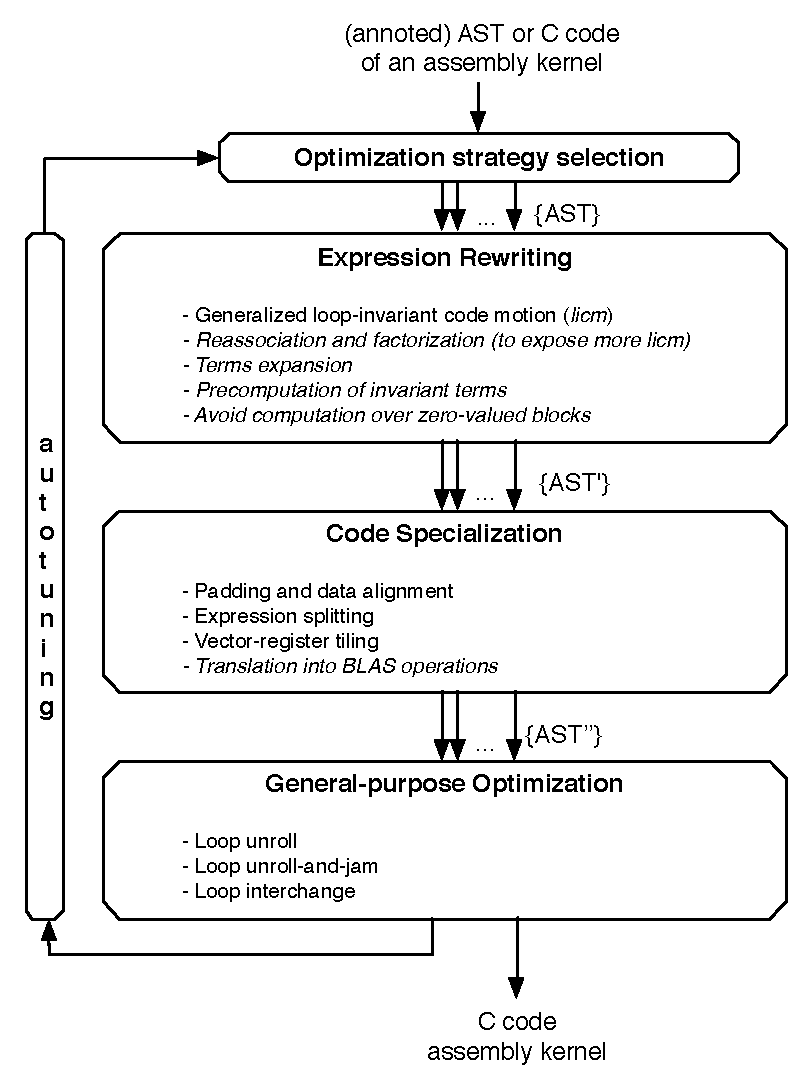
\includegraphics[scale=0.70]{coffee/pictures/coffee-scheme.pdf}
\caption{Structure of COFFEE.}
\label{fig:coffee-compiler-structure}
\end{center}
\end{figure}

Figure~\ref{fig:coffee-compiler-structure} outlines the various modules composing COFFEE. Expression rewriting, code specialization, and general-purpose transformations are applied by manipulating the AST representing the local assembly kernel. Providing the steps of all algorithms performing the various transformations would just be tedious and marginally helpful for the reader; essentially, implementing a transformation always reduces to write a routine that visits and manipulates a tree data structure (the AST) according to the semantics described in Sections~\ref{sec:coffee-expr-rewrite} and~\ref{sec:coffee-code-spec}. In this section, we rather focus on aspects of the compiler implementation that involve the orchestration of the different transformations, including a description of the data structures employed to track both the restructuring of the assembly expressions and data dependencies. 

%TODO The implementation of all code transformations is centered on analysis and manipulation of the kernel AST

\subsection{Tree Visitors}
...

\subsection{Code Hoisting}
Hoisting is the operation of moving code, for instance a statement or the evaluation of an expression, from an inner to an outer loop in a nest. This operation is performed in several occasions when rewriting an expression: generalized loop-invariant code motion, expansion of sub-expressions, and precomputation of terms all require code hoisting, as illustrated in Figures~\ref{code:invariant-code} and~\ref{code:expanded-code}. In order to perform code hoisting, in particular, several aspects must be known:
\begin{enumerate}
\item ``what'' to hoist
\item ``where'' to hoist (possibly, outside of the loop nest)
\item if scalar-expansion should be introduced
\end{enumerate}
Answers to these three points obviously depend on the specific transformation, although parts of the implementation are shared. COFFEE tracks hoisted code by means of a dictionary that binds variable names (guaranteed to be unique) to a set of information. In particular, for a variable \texttt{v}, the dictionary provides:
\begin{itemize}
\item a reference to the AST node corresponding to the expression \texttt{e} hosted by \texttt{v};
\item a reference to the loop in which \texttt{v} is assigned \texttt{e};
\item a reference to the AST node corresponding to the declaration of \texttt{v}.
\end{itemize}
As expressions are hoisted, the dictionary is populated and/or updated with new information. For example, when applying generalized loop-invariant code motion, a new entry is created, unless the sub-expression being lifted has already been pre-computed elsewhere. On the other hand, when sub-expressions are expanded, either a new entry is created or an old entry is updated, as explained in Section~\ref{sec:coffee-expansion}. 

The dictionary is also queried at code specialization time for padding, data alignment and generation of BLAS calls. Therefore, different algorithms in COFFEE access the same data structure, which allows avoiding both duplicated code and an additional overhead due to revisiting the same portion of AST in distinct transformations.

\subsection{Tracking Data Dependencies}
COFFEE implements ``smart'' code hoisting: everytime a sub-expression or a term are lifted, for example from the mathematical expression evaluating the local element matrix to an outer level in the loop nest, three optimizations are potentially applied. Consider a hoistable expression \texttt{e} assuming different values in the iteration space \texttt{I}:
\begin{itemize}
\item \textbf{Minimize redundant computation.} If an equivalent sub-expression \texttt{e'} has already been hoisted along the iteration space \texttt{I}, then COFFEE replaces \texttt{e} with a reference to the symbol hosting the value of \texttt{e'}. This avoids both redundant computation and the introduction of additional temporary variables;
\item \textbf{Loop fusion.} If scalar-expansion is introduced (we recall this is useful to achieve SIMD auto-vectorization; see Sections~\ref{sec:coffee-licm} and~\ref{sec:coffee-precompute}), then the hoisted code must be placed in an outer loop \texttt{r}, \texttt{r $\in$ I}. This was the purpose of the second \texttt{r} loop in Figure~\ref{code:invariant-code}; note that this loop includes scalar-expanded sub-expressions that, in the non-transformed code, iterated along logically different spaces (loops \texttt{j} and \texttt{k}, corresponding to test and trial functions). In this example, it was possible to use a single \texttt{r} loop because we assumed that test and trial function spaces were the same, leading to identical loop bounds; in general, however, this is not true. Another assumption of the example was that the space of the equation's coefficients (variables \texttt{f0, f1} in the figure) coincided with that of test and trial functions. This would allow fusing the two \texttt{r} loops, which is exactly what COFFEE does, although not displayed by the figure. Fusing loops, which increases data locality and reduces loop overhead, is possible in some circumnstances, in particular when there are no data dependencies among hoisted expressions and the spaces of test, trial, and coefficent functions are identical. As explained next, COFFEE reasons about data dependencies and iteration spaces to determine the safeness of loop fusion.
\item \textbf{Reduce extra memory.} When expanding an expression, terms hoisting is possible to relieve register pressure. This poses the challenge described in Section~\ref{sec:coffee-expansion} and intuitively summarized in Figure~\ref{code:expanded-code}; that is, understanding whether it is possible to absorb the hoistable term in an available temporary value or a new temporary is needed. Obviously, the less is the number of temporaries introduced, the smaller is the size of the working set, which may result in better performance.
\end{itemize}
To implement these optimizations, it is necessary to track the evolution of data dependencies as the assembly expression is rewritten. For this purpose, COFFEE uses a dependency graph, which is a standard approach used by general-purpose compilers relying on abstract syntax trees (in addition to other data structures) as intermediate representation. The dependency graph has as many nodes as the number of variables in the loop nest characterizing the assembly expression. A direct edge from a node \texttt{A} to a node \texttt{B} indicates that the value of symbol \texttt{B} depends on that of \texttt{A}. 

The implementation of the depedency graph data structure and of the various algorithms using it is made simple by the fact that COFFEE ensures \textit{static single assignment} form. This property, typically adopted by intermediate representations in compilers, requires that variables are assigned exactly once, and that each variable is defined in advance. 

\subsection{Handling Corner Cases}
Any possible corner cases are handled: for example, if outer-product vectorization is to be applied but the size of the iteration space is not a multiple of the vector length, then a remainder loop, amenable to auto-vectorization, is inserted (as shown in Figure~\ref{code:burgers-opvect}).